% Created 2023-04-02 Sun 21:54
% Intended LaTeX compiler: pdflatex
\documentclass[11pt]{article}
\usepackage[utf8]{inputenc}
\usepackage[T1]{fontenc}
\usepackage{graphicx}
\usepackage{longtable}
\usepackage{wrapfig}
\usepackage{rotating}
\usepackage[normalem]{ulem}
\usepackage{amsmath}
\usepackage{amssymb}
\usepackage{capt-of}
\usepackage{hyperref}
\graphicspath{{../../books/}}
% TIPS
% \substack{a\\b} for multiple lines text





% pdfplots will load xolor automatically without option
\usepackage[dvipsnames]{xcolor}

\usepackage{forest}
% two-line text in node by [two \\ lines]
% \begin{forest} qtree, [..] \end{forest}
\forestset{
  qtree/.style={
    baseline,
    for tree={
      parent anchor=south,
      child anchor=north,
      align=center,
      inner sep=1pt,
    }}}
%\usepackage{flexisym}
% load order of mathtools and mathabx, otherwise conflict overbrace

\usepackage{mathtools}
%\usepackage{fourier}
\usepackage{pgfplots}
\usepackage{amsthm, mathabx,  amsmath, commath}
\usepackage{amsfonts}

\usepackage{empheq}
\usepackage{tikz}
\usetikzlibrary{arrows.meta}
\usepackage[most]{tcolorbox}

\newtheorem{theorem}{Theorem}[section]
\newtheorem{definition}{Definition}[section]
\newtheorem{corollary}{Corollary}[section]
\newtheorem{example}{Example}[section]
\newtheorem{lemma}{Lemma}[section]
\newtheorem{proposition}{Proposition}[section]

\newcommand{\bl}[1] {\boldsymbol{#1}}
\newcommand{\Wt}[1] {\stackrel{\sim}{\smash{#1}\rule{0pt}{1.1ex}}}
\newcommand{\wt}[1] {\widetilde{#1}}


%For boxed texts in align, use Aboxed{}
%otherwise use boxed{}

\DeclareMathSymbol{\widehatsym}{\mathord}{largesymbols}{"62}
\newcommand\lowerwidehatsym{%
  \text{\smash{\raisebox{-1.3ex}{%
    $\widehatsym$}}}}
\newcommand\fixwidehat[1]{%
  \mathchoice
    {\accentset{\displaystyle\lowerwidehatsym}{#1}}
    {\accentset{\textstyle\lowerwidehatsym}{#1}}
    {\accentset{\scriptstyle\lowerwidehatsym}{#1}}
    {\accentset{\scriptscriptstyle\lowerwidehatsym}{#1}}
}

\usepackage{graphicx}
    
% text on arrow for xRightarrow
\makeatletter
%\newcommand{\xRightarrow}[2][]{\ext@arrow 0359\Rightarrowfill@{#1}{#2}}
\makeatother


\def \bx {\boldsymbol{x}}
\def \ba {\boldsymbol{a}}
\def \bI {\boldsymbol{I}}
\def \bt {\boldsymbol{t}}
\def \bb {\boldsymbol{b}}
\def \bA {\boldsymbol{A}}
\def \bX {\boldsymbol{X}}
\def \bu {\boldsymbol{u}}
\def \bS {\boldsymbol{S}}
\def \bZ {\boldsymbol{Z}}
\def \bz {\boldsymbol{z}}
\def \by {\boldsymbol{y}}
\def \bw {\boldsymbol{w}}
\def \bT {\boldsymbol{T}}
\def \bS {\boldsymbol{S}}
\def \bm {\boldsymbol{m}}
\def \bW {\boldsymbol{W}}
\def \bY {\boldsymbol{Y}}
\def \bH {\boldsymbol{H}}
\def \blambda {\boldsymbol{\lambda}}
\def \bPhi {\boldsymbol{\Phi}}
\def \btheta {\boldsymbol{\theta}}
\def \bmu {\boldsymbol{\mu}}
\def \bphi {\boldsymbol{\phi}}
\def \bSigma {\boldsymbol{\Sigma}}
\def \lb {\left\{}
\def \rb {\right\}}
\def \caln {\mathcal{N}}
\def \dissum {\displaystyle\Sigma}
\def \dispro {\displaystyle\prod}
\def \E {\mathbb{E}}
\def \Q {\mathbb{Q}}
\def \V {\mathbb{V}}
\def \R {\mathbb{R}}
\def \calq {\mathcal{Q}}
\def \calg {\mathcal{G}}
\def \caln {\mathcal{N}}
\def \calr {\mathcal{R}}
\def \calm {\mathcal{M}}
\def \calc {\mathcal{C}}
\def \bcup {\bigcup}

\makeindex
\author{Martin Kleppmann}
\date{\today}
\title{Distributive Systems}
\hypersetup{
 pdfauthor={Martin Kleppmann},
 pdftitle={Distributive Systems},
 pdfkeywords={},
 pdfsubject={},
 pdfcreator={Emacs 28.0.92 (Org mode 9.6.1)}, 
 pdflang={English}}
\begin{document}

\maketitle
\tableofcontents

\section{Introduction}
\label{sec:org040af72}
This type of interaction, where code on one node appears to call a function on another node, is
called a \textbf{Remote Procedure Call}.

What if..
\begin{itemize}
\item the service crashes during the function call?
\item a message is lost?
\item a message is delayed?
\item something goes wrong, is it safe to retry?
\end{itemize}

Today, the most common form of RPC is implemented using JSON data sent over HTTP. A popular set
of design principles for such HTTP-based APIs is known as \textbf{representational state transfer} or
\textbf{REST} , and APIs that adhere to these principles are called \textbf{RESTful}. These
principles include:
\begin{itemize}
\item communication is stateless (each request is self-contained and independent from other requests)
\item resources (objects that can be inspected and manipulated) are represented by URLs
\item the state of a resource is updated by making a HTTP request with a standard method type, such
as \texttt{POST} or \texttt{PUT}, to the appropriate URL.
\end{itemize}
\section{Models of distributed systems}
\label{sec:orgb1f3373}
\subsection{The two generals problem}
\label{sec:org07f8c08}
In the two generals problem, we imagine two generals, each leading an army, who
want to capture a city. The city’s defences are strong, and if only one of the two armies
attacks, the army will be defeated. However, if both armies attack at the same time, they will
successfully capture the city.

Thus, the two generals need to coordinate their attack plan. This is made difficult by the fact
that the two armies are camped some distance apart, and they can only communicate by messenger.
The messengers must pass through territory controlled by the city, and so they are sometimes
captured. Thus, a message sent by one general may or may not be received by the other general,
and the sender does not know whether their message got through, except by receiving an explicit
reply from the other party. If a general does not receive any messages, it is impossible to tell
whether this is because the other general didn’t send any messages, or because all messengers
were captured.1

\begin{center}
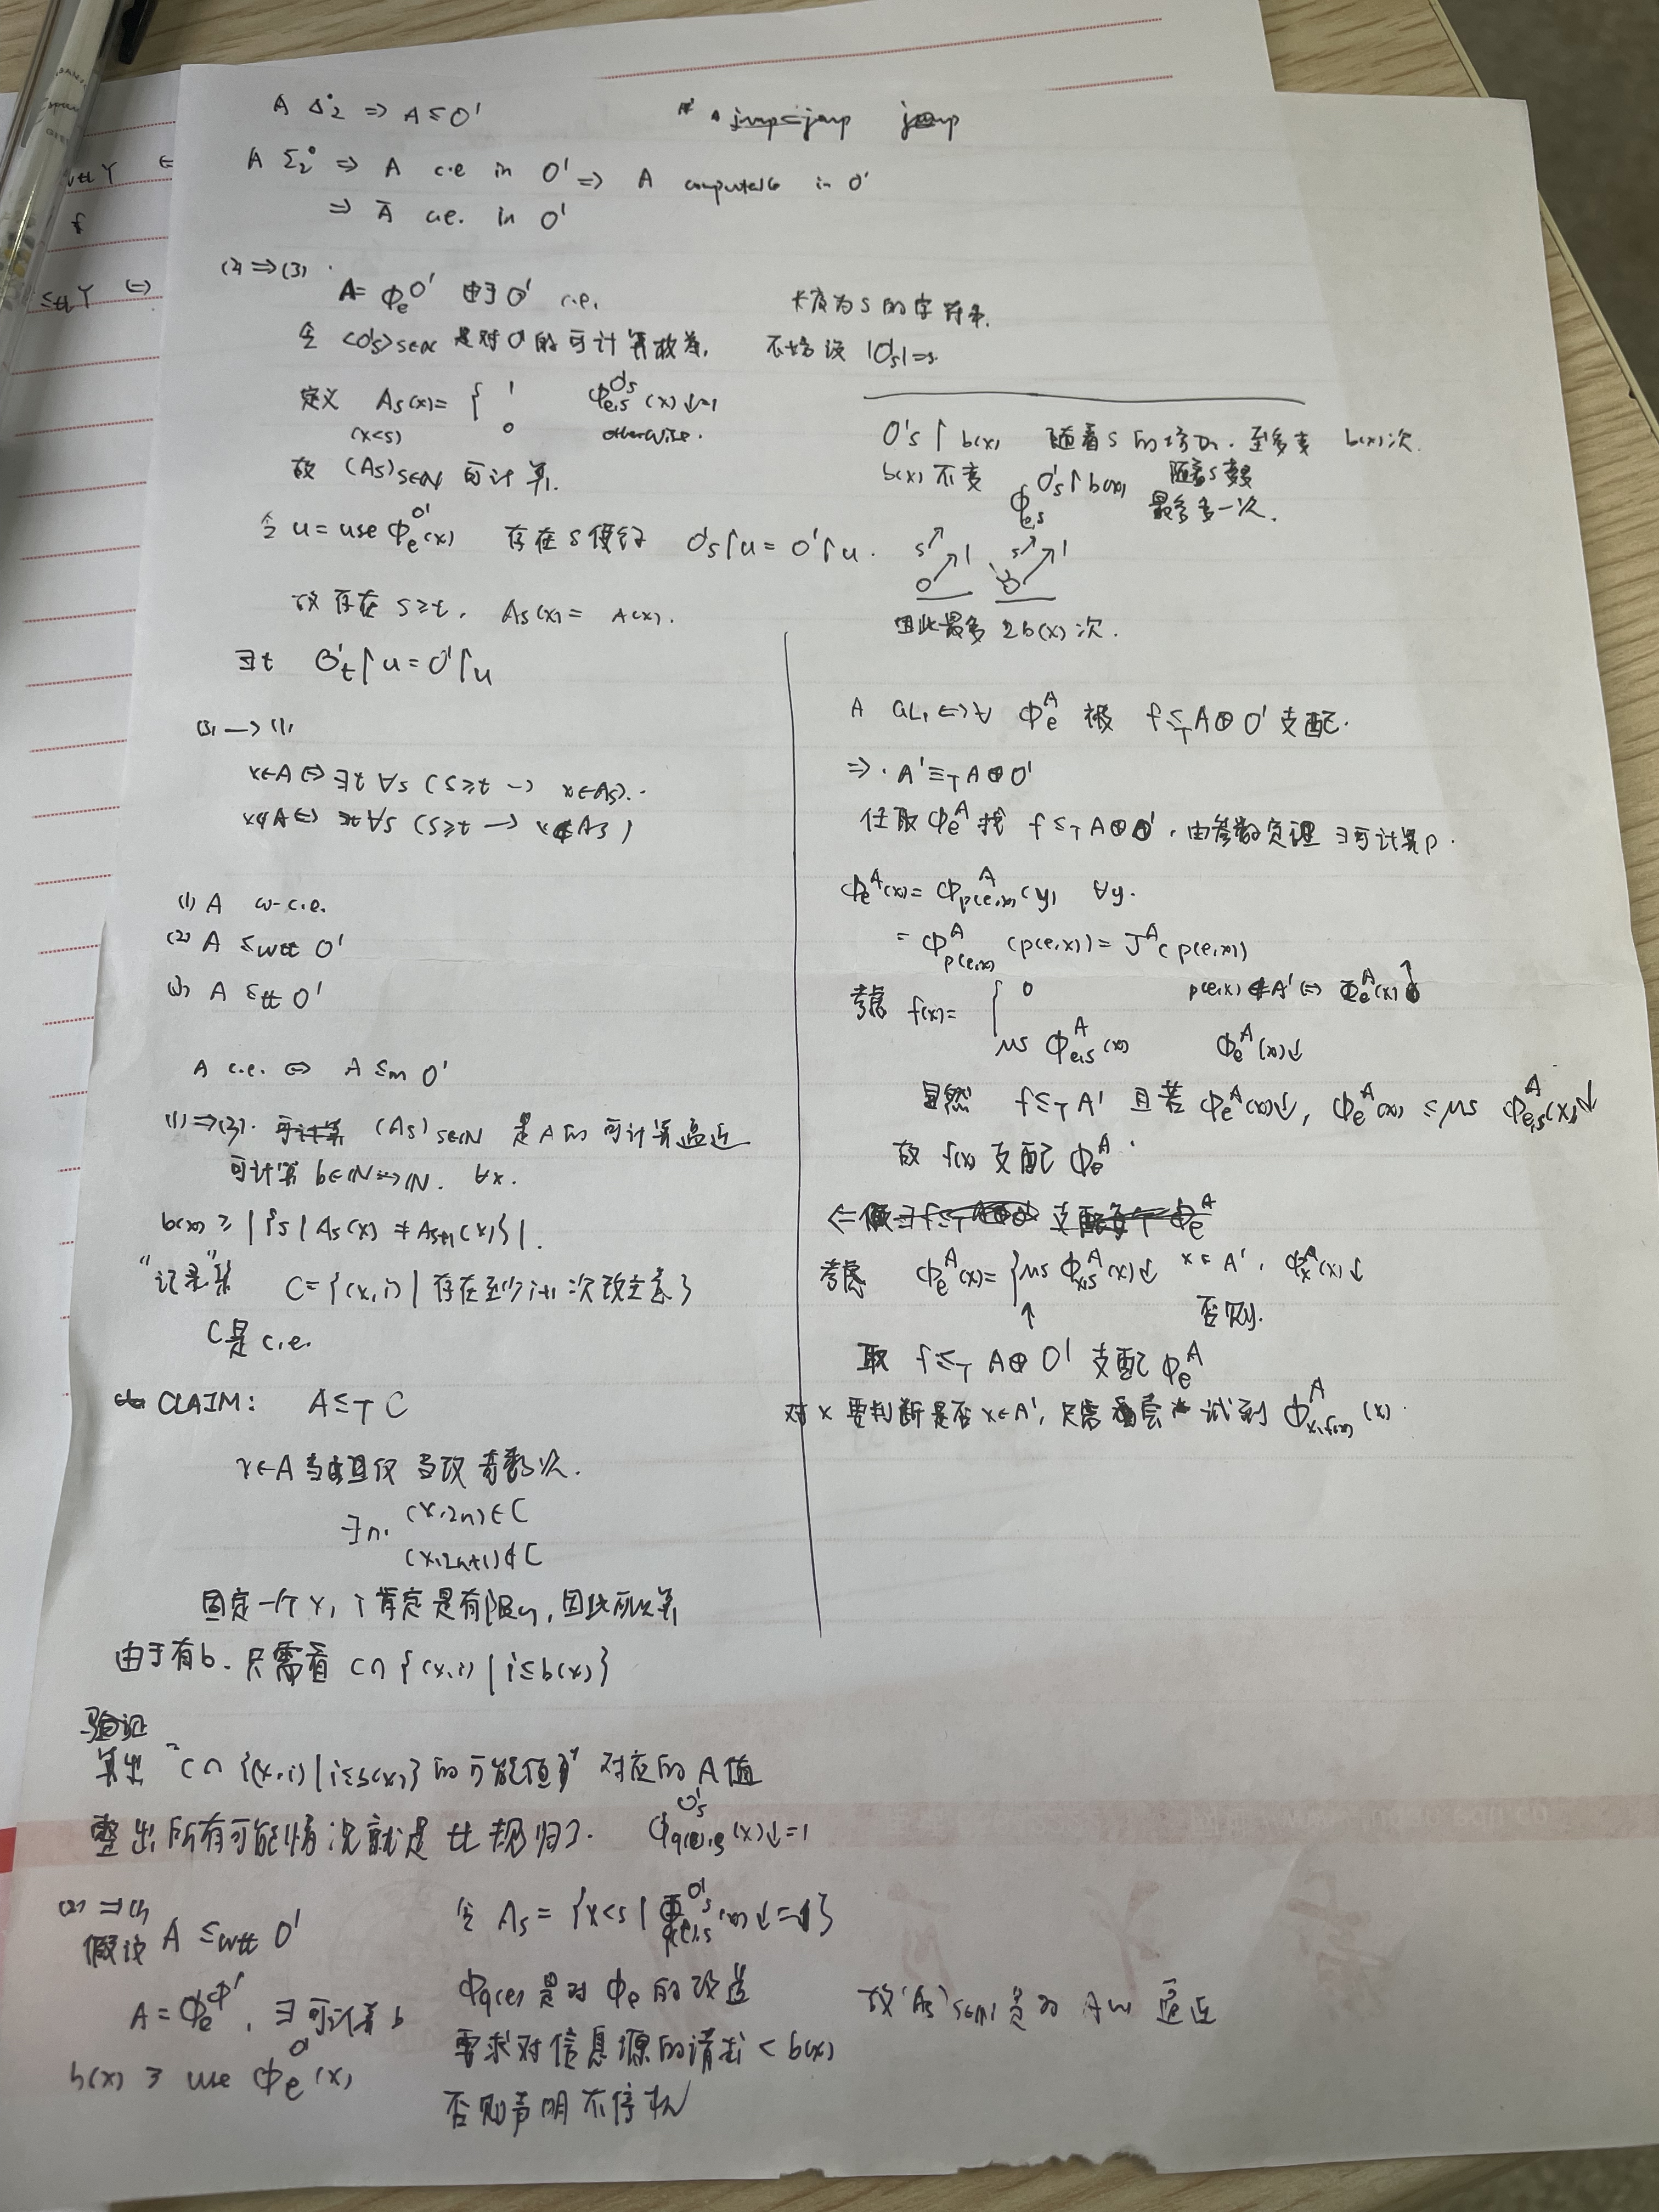
\includegraphics[width=.7\textwidth]{../images/DistributiveSystems/1.png}
\label{}
\end{center}

How should the generals decide?
\begin{enumerate}
\item General 1 always attacks, even if no response is received?
\begin{itemize}
\item send lots of messengers to increase probability that one will get through
\item if all are captured, general 2 does not know about the the attack, so general 1 loses
\end{itemize}
\item General 1 only attacks if positive response from general 2 is received?
\begin{itemize}
\item Now general 1 is safe
\item But general 2 knows that general 1 will only attack if general 2's response gets through
\item now general 2 is in the same situation as general 1 in option 1
\end{itemize}
\end{enumerate}
\textbf{No common knowledge}: the only way of knowing something is to communicate it

The problem is that no matter how many messages are exchanged, neither general can ever be
certain that the other army will also turn up at the same time. A repeated sequence of
back-and-forth acknowledgements can build up gradually increasing confidence that the generals
are in agreement, but it can be proved that they cannot reach certainty by exchanging any finite
number of messages.
\subsection{The Byzantine generals problem}
\label{sec:org4a29bee}
We have armies wanting to capture a city, though in this case there can be three or more. Again
generals communicate by messengers, although this time we assume that if a message is sent, it
is always delivered correctly.

\begin{center}
\includegraphics[width=.7\textwidth]{../images/DistributiveSystems/2.png}
\label{}
\end{center}

The challenge in the Byzantine setting is that some generals might be “traitors”: that is, they
might try to deliberately and maliciously mislead and confuse the other generals. We call the
traitors \textbf{malicious}, and the others \textbf{honest}.

\begin{center}
\includegraphics[width=.7\textwidth]{../images/DistributiveSystems/3.png}
\label{}
\end{center}
\begin{theorem}[]
Need \(3f+1\) generals in total to tolerate \(f\) malicious generals
\end{theorem}

\begin{center}
\includegraphics[width=.6\textwidth]{../images/DistributiveSystems/4.png}
\label{}
\end{center}

In distributed systems, some systems explicitly deal with the possibility that some nodes may be
controlled by a malicious actor, and such systems are called \textbf{Byzantine fault tolerant}.
\subsection{Describing nodes and network behaviour}
\label{sec:orge1df0cc}
\begin{itemize}
\item Two generals problem: a model of networks
\item Byzantine generals problem: a model of node behaviour
\end{itemize}

Capture assumptions in a \textbf{system model} consisting of
\begin{itemize}
\item network behaviour
\item node behaviour
\item timing behaviour
\end{itemize}

\textbf{Network behaviour}: Assume bidirectional \textbf{point-to-point} communication between two nodes with one
of:
\begin{itemize}
\item \textbf{Reliable} (perfect) links:
\begin{itemize}
\item A message is received iff it is sent.
\item Message may be reordered.
\end{itemize}
\item \textbf{Fair-loss} links:
\begin{itemize}
\item Messages may be lost, duplicated, or reordered
\item If you keep retrying, a message eventually gets through
\end{itemize}
\item \textbf{Arbitrary} links:
\begin{itemize}
\item A malicious adversary may interfere with messages
\end{itemize}
\end{itemize}

\begin{center}\begin{tikzcd}
Arbitrary\ar[r,"\text{TLS}"]&Fair-loss\ar[r,"\text{retry+dedup}"]&Reliable
\end{tikzcd}\end{center}
\end{document}